\documentclass[10pt,twocolumn]{article}
\usepackage{cite}
\usepackage{graphicx}
\usepackage{pdfpages}
\usepackage{rotating}
\usepackage{placeins}
\usepackage{csvsimple}
\usepackage{listings}
\usepackage{url}
\usepackage{amsmath}
\usepackage{stmaryrd}
\newcommand*\concat{\mathbin{\|}}
\usepackage{siunitx}
\usepackage{booktabs}
\usepackage{xcolor}
\pagestyle{plain}

\providecommand{\keywords}[1]{\textbf{\textit{Index terms---}} #1}

\begin{document}

\title{Mini-MAC: Raising the Bar for Vehicular Security\\
with a Lightweght Message Authentication Protocol}

%\author{Redacted for anonymous submission}

\author{Jackson Schmandt,$^1$
Alan T. Sherman,$^2$ 
Nilanjan Banerjee$^1$\\
CSEE Department, University of Maryland, Baltimore County (UMBC)\\
\{schmandt, sherman, nilanb\}@umbc.edu\\}

\date{\today}

\maketitle

\footnotetext[1]{Mobile Pervasive Sensor System Lab}
\footnotetext[2]{Cyber Defense Lab}

\begin{abstract} % 199 words

We propose Mini-MAC, a new message authentication protocol that works in 
existing automotive computer networks without adding any bus overhead. 

Deployed in many vehicles, the CAN bus is a low-speed network connecting electronic control units,
including those that control critical functionality such as braking and acceleration.  
The CAN bus is extremely vulnerable to malicious actors with bus access. Traditionally, 
Message Authentication Codes (MACs) help authenticate the sender of a message, 
and variants prevent message replay attacks; however, 
standard MACs are unsuitable for use on the CAN bus because of small payload sizes. 
Restrictions of the CAN bus, including the need not to delay messages,  
severely limit how well this network can be protected.
%Do we need to clarify  why the CAN bus is vulnerable here?
%I don't think time-seeding has an impact on the suitability of a MAC for the CAN bus

Mini-MAC is based on a counter-seeded HMAC, augmented with message history and truncated to fit available message space. 
It causes no increase in bus traffic and incurs a very small performance penalty relative to the provably secure HMAC. 
It is the first proposal to combine these two tenets for vehicle networks. 
Even though the CAN bus cannot be properly secured against a dedicated attacker, 
Mini-MAC meaningfully raises the bar of vehicular security, enhancing the safety of drivers and
others.

%and the proposed Car-to-X environment.

\end{abstract}

\keywords{CAN bus,
	automotive security,
	message authentication code,


	Mini-MAC,
	vehicle security,
	applied cryptography.
}

\section{Introduction}
\label{intro}

At the 2015 Black Hat conference, Miller and Valasek~\cite{blackhat} gained full control of a new Jeep,
including its engine, brakes, and steering, by exploiting vulnerabilities in its
computer network and Wi-Fi implementation and by rewriting firmware on a controller connected to the car's entertainment system.
This demonstration, and other similar 
projects~\cite{Rouf2010,Koscher-2010,Checkoway-2011,Woo-14,C2X}, 
highlight the egregious state of vehicular security, including the lack of 
authentication of messages sent on the Controller Area Network (CAN).   

To strengthen vehicular security in a simple and practical 
yet meaningful way---without replacing the CAN bus---we propose Mini-MAC, 
a new variable-length Message Authentication Code (MAC)
for the CAN bus that works with small payload sizes without delaying messages.  
Mini-MAC is an authentication component that can be an important part of a larger system solution
to enhance vehicular security.

Built on the provably-secure HMAC, Mini-MAC protects against masquerade attacks.  
Mini-MAC also incorporates a counter and message history to protect against replay attacks;
the message history feature protects against all transient attackers (attackers
who can access the CAN bus only for a limited period of time).
To avoid sending separate messages to different recipients, Mini-MAC applies authentication keys
shared among groups of communicating Electronic Control Units (ECUs).
It is the first proposal to authenticate messages on the CAN bus without increasing bus traffic
or delaying messages. 

Traditional authentication protocols (including digital signatures or full-length MACs) are unsuited for the CAN bus due to
small packet size, limited computational power of the ECUs,
and the need not to delay messages (e.g., by time-consuming computations or by
increasing bus traffic).   

Mini-MAC improves on previous proposals, including Lin-MAC~\cite{Lin-MAC}, by not increasing bus traffic.
Furthermore, Mini-MAC is easy to implement,
requires no fundamental change to the underlying functionality of the ECUs, and 
requires no special hardware.

Our work includes a prototype implementation of Mini-MAC and preliminary timing studies 
of Mini-MAC for three component hash functions (MD5, SHA-1, SHA-2).  
In comparison with a straight-forward HMAC, our Mini-MAC implementations show on average
a mean code size increase of 5.99\% and 
a mean execution time increase of only 2.58\%.
For fastest speeds, we recommend using mini-MAC-MD5, for which our implementation 
running on an 8~MHz processor takes on average 
7.5 milliseconds~(ms) to compute a tag.

Our contributions include:
\begin{itemize}

\item Mini-MAC, an authentication protocol suitable for many vehicular systems, including the CAN bus, 
that require short message sizes and no message delays.
Mini-MAC meaningfully raises the bar on authentication strength for the CAN bus, protecting against
masquerade and replay attacks.

\item Mini-MAC's use of message history protects against all transient attackers, 
even if they know the keys.

\item Experimental demonstration of Mini-Mac, including execution times of Mini-MAC 
with each of three HMAC implementations using the MD5, SHA-1, and SHA-2 hash functions. 
On average our implementation of Mini-MAC-MD5 takes 7.5~ms to compute a tag.

\end{itemize}


\section{Background}
\label{background}

This section briefly reviews essential background on vehicular security and message authentication codes. 
The experienced reader may wish to skip to Section~\ref{problem}. 
We assume the reader is familiar with cryptographic hash functions as explained, for example, by Stinson~\cite{Sti} and NIST~\cite{FIPS-180-4}.
\textcolor{red}{Note: You mentioned Stinson on the last draft notes -- this is the book Cryptography - Theory and Practice?---YES}.

\subsection{ECUs}
The Electronic Control Units (ECUs) found in an automotive computer network are low-power, single-purpose devices. ECUs on the CAN bus control many components in a modern automobile, from headlights and window controls, to brakes and engine. They are not typically designed with security in mind and frequently comprise a basic CAN bus transceiver, basic message processor, and an actuator. The message processor identifies whether or not a message being broadcast is interesting to the ECU and arbitrates bus rights with the other ECUs. 

\subsection{The CAN Bus}
The CAN bus is a simple, low-speed bus designed to network simple nodes. In an automotive environment, 
it typically runs at 500~kbps.\footnote{kilobits per second (kbs).} As shown in Figure~\ref{fig-frame}, 
a frame contains an 11-bit identifier field and 
a data payload, as well as some control bits. Figure~\ref{fig-frame} shows the data payload as 8~bits, but
it can be 8 to 64~bits and is typically 64~bits. [ref?]
The payload of up to 8~bytes is the most important element, as any MAC must fit into this frame or use a more complex multi-frame data transmission protocol that may or may not be supported on all ECUs. 

We use the term ``message'' to refer to the data payload (of up to 64~bits) in one frame.
Any payload longer than 64~bits must be sent as a multi-frame transmission.
[do we want multi-frame message, or multi-frame/multi-message transmission?]

% we need agreement on terminology.  Do we instead want to use "multi-frame message" ?
% is there an industry convention?

Ideally, and in the case of Mini-MAC, the MAC can fit into the payload with the data, thus not increasing bus utilization. Data captured by the authors from a 2010 Toyota Prius show that a large percent (61\%) of messages use no more than four bytes of data in the payload.
We observed approximately 25 messages sent per second on average (40 maximum per second).

% On the diagram, there are 55 bits including 8 data bits. In practice, the 8 bit field is 64 bits, 
% so the total packet is 111 bits. So there are more than 64 total bits sent, but not more than 64 data bits.

%The "frame" is the entire transmission put onto the CAN bus -- this includes 47b of wrapper (ID, CRC and some control bits) and up to 64b of data (observed %packets are all 64b). Some of the control bits are used to indicate the size of the data field -- in the diagram used, the data field is only 8 bits, but %the size of this is variable (up to 64 bits) and indicated in the header of the frame.
%A "message," as I have used it, is the contents of the data field being send from one ECU to another. I think of it as what an application layer would %generate on one ECU and what the application layer in another ECU would receive.

	\begin{figure*}
		\centering
		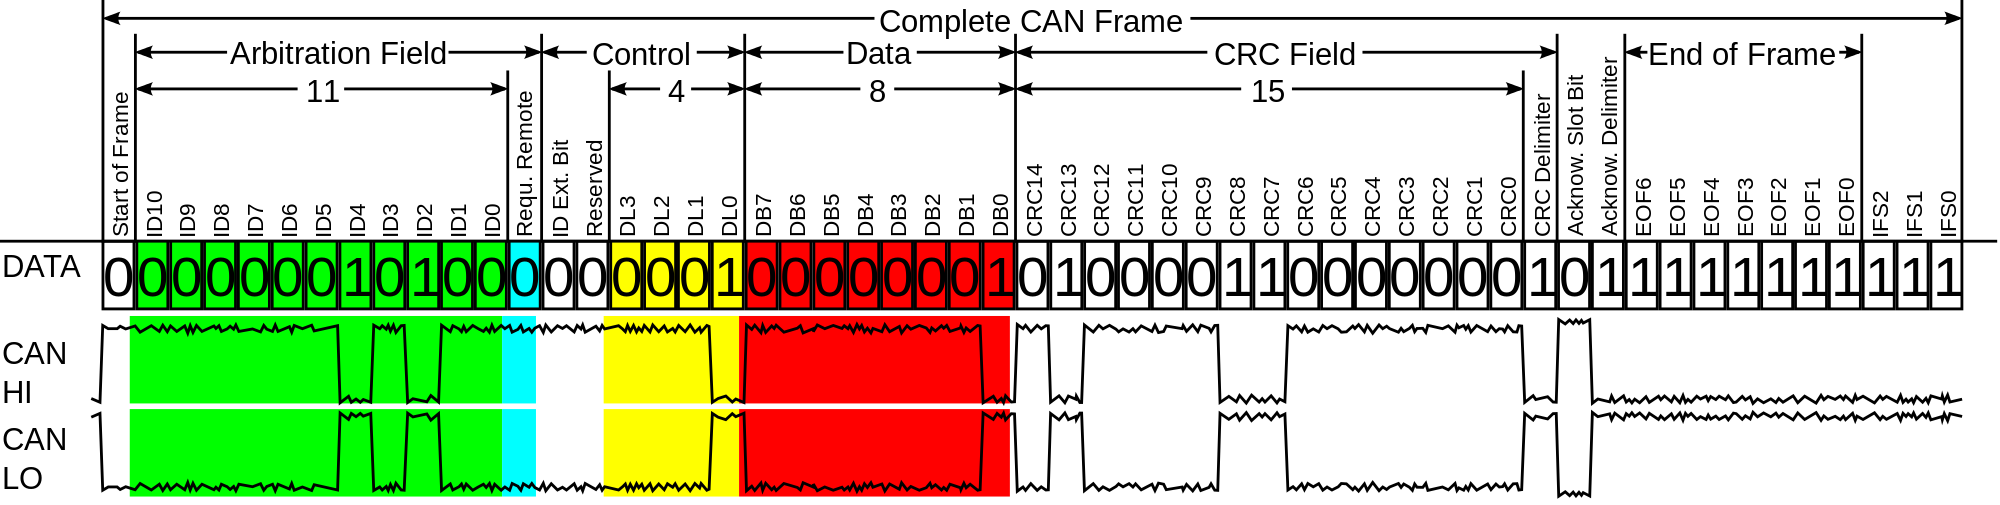
\includegraphics[width=\linewidth]{figures/can_frame.png}
		\caption{The CAN frame~\cite{} [need to cite fig].  
		Each message on the CAN bus is a structured sequence of 55--111~bits including 8--64 data~bits.}
		\label{fig-frame}
	\end{figure*}

\subsection{Bus Access}

To spoof or replay messages on the CAN bus, the attacker must have access to it.
There are several ways to access the CAN bus:  (1) There is a
physical connection through the On-Board Diagnostic (OBD-II) port, 
typically located underneath the steering wheel.  An attacker might hide
access to this port by splicing into unexposed wires.
(2) An attacker might corrupt an ECU by rewriting its firmware. An attacker might
do so while the car is being serviced or by entering the car while it is parked.
(3) An attacker might gain access to the CAN bus by exploiting or corrupting a peripheral
device connected to it, such as a cellular phone, audio system, or Bluetooth
radio.  For example, Checkowa~\cite{Checkoway-2011} gained bus access by packing 
malware into a WMA audio file played on the car stereo. [give another example
of wireless access from drive-by attacker]

Despite many demonstrated security flaws, automotive 
manufacturers have been unreasomnably hesitant to acknowledge the vulnerabilities inherent to the CAN bus,
sometimes wishfully claiming that undetected bus access is difficult. [do you have a cite? for example,
a quote from a car manufacturer saying something ridiculous?]

\subsection{Message Authentication Codes}

Given a message and optionally a key, a Message Authentication Code (MAC) computes a short string (called a tag) 
that a recipient can use, together with the message, to verify the authenticity of the message.  The recipient 
verifies the tag by recomputing it.

The Keyed-Hash Message Authentication Code (HMAC)~\cite{HMAC,FIPS-198-1} 
is a well-known MAC construction that keys an underlying component hash function.  
Breaking it is as hard as breaking the component hash function.

HMAC is computed as

\begin{equation}
H((k\oplus \text{opad})\concat H((k\oplus \text{ipad})\concat \text{message}) ,
\end{equation}

\noindent
where $k$ is the key, and opad and ipad are the outer and inner hash padding strings, respectively. 
These strings are constant strings defined by 0x5C and 0x36, repeated until the hash input is of the appropriate length. 
$H$ is the component hash function used. 
The symbols $\oplus$ and $\concat$ represent XOR and concatenation, respectively.\footnote{Exclusive-or (XOR).}

%\subsection{Car-to-X}




\section{Problem Statement}
%Say the task is to create an authentication mechanism that
%(list requirements): time, space, securit, etc
%rewrite the problem statement

The task of this work is to create an authentication mechanism suitable for use on the CAN bus in vehicular environments. Given the context, this mechanism must provide some measurable increase in security over the standard non-secured bus. It must not increase bus traffic, and it must not violate message delay constraints. Additionally, the mechanism must provide protection from replay and masquerade attacks as defined in Section 5.

In test data captured by the authors for a 2010 Toyota Prius, over 60\% of messages contain no more than four data bytes. This usually leaves four bytes of space for a MAC.

The ECUs in a car are slow, low-power systems incapable of complex cryptographic functions. Given these limitations, the problem addressed is how to add as much security as possible without breaking the system.


\section{Previous Work}
\label{previous}

Previous proposals to add authentication to the CAN bus violate the engineering constraints described
in Section~\ref{problem}, increasing bus traffic and delaying messages.  For example, pairwise
key distribution among the ECUs and data that overflow CAN frame boundaries cause additional messages to be sent,
delaying messages.

For example, Lin and Sangiovanni~\cite{Lin-MAC} propose Lin-MAC, a keyed MAC with counter based on
pairwise key distribution.  Encrypting the same message to $n$ different ECUs requires $n$
messages to be sent.   Using the full HMAC-MD5 requires 128~bits to be sent per message, requiring two CAN frames per message.

Other recent CAN security projects suffer from similar limitations. 
Woo et al.~\cite{Woo-14} propose a keyed MAC based on pairwise key distribution,
packing the tag into the extended ID field (not used by all ECUs) and the CRC field in the CAN trailer
(for a related proposal of ours, see Section~\ref{addingbits}). 
These bits fit only if the ECUs use the extended ID field. 
Their proposal requires a hardware redesign of CAN transceivers or rewriting a layer of message transmission firmware.
Care should be taken when comparing their computation times because
they assume a much more powerful message processor than we do. 

Zalman and Mayer~\cite{Zalman-14} propose a fixed-size, time-stamped MAC based on pairwise key distribution.
Their tag overflows the CAN frame, increasing bus traffic, and as the authors acknowledge,
delaying messages.

Xie et al.~\cite{Xie-15} propose packing multiple messages into one CAN frame using a keyed MAC with 
pairwise key distribution.   They unrealistically assume that the messages and MAC tag are short
enough to fit into one frame.  Also, by queuing messages into batches, their system delays messages.

%redacted 

Schmandt first worked on the problem in spring 2015
as a research project for Sherman's CMSC-652 cryptology class at UMBC.
Unknown to us until recently, independently, Bravo et al.~\cite{MIT2015} carried out a similar effort 
for Rivest's 6.857 computer and network security class at MIT.  Both projects use HMACs, but in different ways.
The MIT project, assuming lossless channels, initializes each channel with a precomputed HMAC chain.
Using a software CAN bus simulator, they show that their scheme increases message latency by
approximately a factor of three, and increases bus traffic.  By contrast, our method does not increase
bus traffic and does not increase message latency, and our use of message history protects against transient
attackers who know the keys.

%[do we want to cite any other works on improving car security? If so, do it here.]

Many automakers and parts manufacturers are now members of the 
Open Alliance,\footnote{http://www.opensig.org}
a non-profit group researching and encouraging the use of an Ethernet-based high-speed physical layer 
for use in vehicles.  This approach would enable the use of 
established network security mechanisms in vehicle networks.




\section{Adversarial Model}
\label{adversary}

We consider three classes of adversaries:

\begin{description}

	\item [Type 1]
	(\textit{Strongest adversary}): A permanent entity on the CAN bus with a valid key for the MAC it wishes to generate.
	
	\item [Type 2]
	(\textit{Strong adversary}): A permanent entity on the CAN bus without a valid key for the MAC it wishes to generate.
	
	\item [Type 3]
	(\textit{Weak adversary}): A transient entity on the CAN bus without a valid key for the MAC it wishes to generate.
	
\end{description}

For example, a Type~1 adversary might be a compromised ECU on the CAN bus.  A Type~2 adversary might be a malicious piece of hardware attached
to the CAN bus.  A Type~3 adversary might be a criminal who has gained temporary access to the CAN bus, perhaps via a wireless channel from
another nearby car.  For a Type~3 attacker, we assume the adversary's access to the CAN bus is limited to minutes, not hours.  
The differences among these attackers are what keys they know and for how long they have access to the CAN bus.
This project aims to defend against Type~2 and Type~3 adversaries.   Our techniques do not protect against 
a Type~1 adversary, who can spoof any message to any member of any group to which he holds the key. 

Motivation of the attacker includes criminal mischief (e.g., crashing car, destroying property) and theft.  
For example, spoofing messages on the CAN bus can unlock doors, disable brakes, and accelerate the car.
Goals of the attacker include spoofing or replaying messages on the CAN bus that will be accepted by an ECU
as valid.

We assume the attacker posses complete knowledge of the CAN bus and ECUs, including all protocols, message IDs, and formats.
We assume the attacker has substantial computing power, reliable access to the CAN bus, and is able to 
monitor and inject messages on the bus.  We assume, however, that the adversary cannot inject more than 40 messages
per second without detection.

We assume the ECUs are trustworthy and that the adversary cannot break standard cryptographic functions 
including encryption and hash functions.

This work does not address Denial-of-Service (DOS) attacks aimed at preventing a driver from using her vehicle.  
For example, our techniques do not prevent an attacker from flooding the CAN bus with messages.  There are many
simple physical DOS attacks, such as slashing a tire, cutting wiring, or draining fuel, yet
a DOS attack on the CAN bus while the vehicle is operating could be dangerous 
(e.g., losing control on high-speed turn).  Guarding against DOS attacks is difficult and would require fundamental
changes to the CAN bus.\footnote{Another potential DOS attack is to radiate the vehicle with an electro-magnetic pulse.
Doing so might be useful to law enforcement in extreme circumstances to stop certain dangerous high-speed criminals, 
if the pulse could be directed in a controlled, focused, and well-targeted manner.}

Although we assume the adversary has complete knowledge of the target technology, in practice the adversary must
deal with the straightforward yet cumbersome task of learning this technology, which may include new ECUs and message formats.




\section{Mini-MAC}
\label{mini-mac}

Mini-MAC is a group-keyed lightweight variable-length truncated HMAC that
depends on a counter and on recent message history.  It does not increase
bus traffic or delay messages.  We explain Mini-MAC in three layers
of abstraction: architecture, design, and  implementation.

[I think we should redesign mini-MAC without counter truncation,
and putting XOR of counter and history before HMAC.]

\subsection{Architecture}
\label{arch}

Four core architectural elements characterize Mini-MAC:
(1)~Variable-size output to fit available space in the CAN packet.
(2)~Shared keys among groups of ECUs to avoid increasing bus traffic.
(3)~A counter to mitigate replay attacks;  also used [for no good reason]
to truncate HMAC outputs.
(4)~Message history to serve as "salt" against possible unknown precomputation attacks. 
[I dislike justifying history on basis of replay because it adds nothing over counter
in that regard.]
Elements (1) and (2) trade authentication strength for performance;  see
Section~\ref{security} for a discussion of this tradeoff.

[even if we keep the "split counter" (which I dislike), there is no need to 
refer to it as such. Simpler is to call it a counter and to derive various
bits from it.]

To avoid sending long tags using additional messages, Mini-MAC truncates the
HMAC to fit available space in the CAN frame (typically the resulting tag is
approximately four bytes).  

To avoid increasing bus traffic by separately authenticating the same message to different recipients, 
Mini-MAC uses long-term shared group keys instead of pairwise keys.  For example, in Figure~\ref{fig-key}, ECUs
2, 3, and 4 share the group key~$k_3$.
Group key distribution is possible because, at system design, the designer knows which ECUs communicate with which others. 
There is no need for a dynamic group key update capability because group membership will never change.
[Keys can be updated by a security manager as needed or desired.(?)]

Using a counter is a simple, standard, and effective way to mitigate replay attacks.  

Each ECU saves recent messages sent on the bus and XORs them into the HMAC input. 
[is this done uniformly by all, or per key group?] 
There are two reasons for this architectual element:  First, 
the history adds an unpredictable ``salt'' that might mitigate some possible
precomputation attacks.  Second, it adds protection against any transient
attacker (even one who knows the group keys) who cannot deduce enough of the 
message history.  It also adds an additional layer of protection 
beyond the counter against replay attacks [this reason is weak and perhaps should therefore be dropped].
	
	\begin{figure}
		\centering
		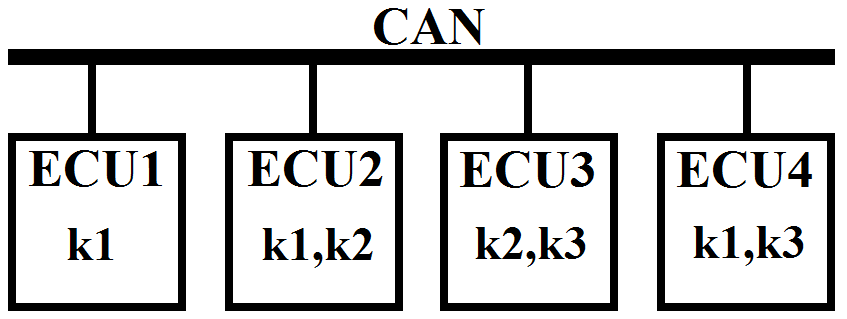
\includegraphics[width=\columnwidth]{figures/key_distribution.png}
		\caption{Mini-MAC key distribution.  Each group of ECUs shares an authentication key.}
		\label{fig-key}
	\end{figure}
	
\subsection{Design}
\label{design}

	\begin{figure}
		\centering
		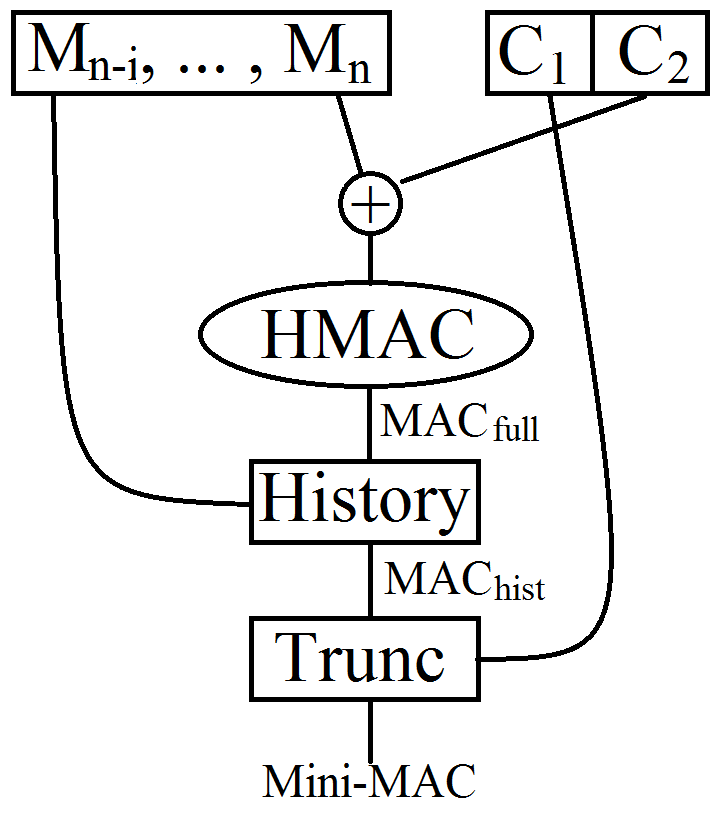
\includegraphics[width=\columnwidth]{figures/minimac_diagram.png}
		\caption{Mini-MAC. The Mini-MAC of a message $M_n$ is a truncated HMAC of 
		the XOR of $M_n$, a counter, and the most recent $i$ messages.}
		\label{fig-minimac}
	\end{figure}

Figure~\ref{fig-minimac} shows how to compute 
$Mini\hbox{-}MAC(k,M_n,s,C,\hbox{History})$, 
where $k$ is the group key, 
$M_n$ is the current message, 
$s$ is the number of available bits in the current CAN frame, 
$C$ is the message counter, 
and $\hbox{History} = (M_{n-i}, \ldots, M_{n-1})$ is the sequence of the most recent
$i$ messages.

The Mini-MAC tag is computed as

\begin{equation}
\text{MAC}_{\text{mini}} = \hbox{trunc(}s,\text{HMAC}(k,\text{Input})),
\end{equation}

\noindent where HMAC is the underlying HMAC and $\hbox{trunc}(s,\cdot)$
extracts $s$ bits from its input.  The input to HMAC is computed as

\begin{equation}
\text{Input} = M_n \oplus C \oplus (M_{n-i} \oplus \cdots \oplus M_{n-1}) .
\end{equation}


%\begin{equation}
%\text{For }i=1:h\text{, MAC}_\text{hist} = \text{MAC}_{\text{full}}\oplus\text{Message}_{n-i}
%\end{equation}
%
%\begin{equation}
%\text{MAC}_{\text{mini}} = \text{MAC}_{\text{full}}(l,l+s)
%\end{equation}


\subsection{Implementation}
\label{implementation}

We implemented Mini-MAC using three different component hash functions (MD5, SHA-1, and SHA-2) to compare the resulting running times.  
Each group key is 128~bits.  The $\hbox{trunc}(s,\cdot)$ function extracts the first $s$ bits of its input. [or explain the obfuscated way]

For \textbf{HMAC-MD5},
we adapted Peslyak's~\cite{Peslyak} implementation of MD5~\cite{MD5} for the MSP430 platform, producing a 128-bit output. 
Despite known collision attacks on MD5~\cite{Wang-MD5}, we consider
MD5 for Mini-MAC for its very fast speed.  [the relevant attack here is known pre-image, not
collision finding.  more in security section]

For \textbf{HMAC-SHA-1},
we adapted Conte's~\cite{Conte-SHA1} SHA-1~\cite{FIPS-180-4} implementation for the MSP430 platform, producing a 160-bit output. 
As for MD5, despite known security vulnerabilities in SHA-1 \cite{Wang-SHA1}, 
we consider SHA1 as a potential candidate.

For \textbf{HMAC-SHA-2},
we also adapted Conte's~\cite{Conte-SHA256} SHA-2-256 implementation for the MSP430 platform, producing a 256-bit output. 
A member of the SHA-2 family of hash functions, SHA-2 is still in use and is recommended by NIST as a cryptographic hash function, 
though SHA-3 will soon replace it\cite{FIPS-180-4}. [check current status of NIST on SHA-2]
[why did we not test SHA-3?]

\section{Testing}
\label{testing}

We measured the execution time and RAM usage of our three Mini-MAC implementations 
running on the Texas Instruments MSP430F5529 microcontroller. 
In speed and power this device is representative of vehicular ECUs.

\subsection{Purpose}
\label{purpose}

The purpose of our tests is to measure the time and space usage of our Mini-MAC implementations, and more generally,
to evaluate the performance suitability of Mini-MAC for authenticating messages on the CAN bus.

\subsection{Methods}
\label{methods}

For each implementation we measured code size, memory usage, execution time, and bus utilization,
collecting for each implementation metrics from 1000 inputs of various typical sizes (1~byte, 2~bytes, 4~bytes).  

We measured code size and RAM usage at compile time using 
the Texas Instruments Code Composer v6.
The RAM usage is know at compile time because there is no
dynamic memory allocation.

We measured execution time using a counter register on the MSP430, 
whose 32~kHz clock provides timing values to approximate millisecond~(ms) accuracy. 
As a very minor point we note that, due to a limitation in the hardware's
support for timing measurements, 
there may be a $\pm$0.03~ms inaccuracy in each reading due to the
time it takes to read the counter.

We collected statistics on message traffic from a 2010 Toyota Prius with a CAN-bus sniffer program 
based on an Arduino Uno platform and connected via an OBD-II CAN transceiver shield.

%\subsection{Results}
%\label{results}
%
%Tables~\ref{tab-traffic}, \ref{tab-overhead}, \ref{tab-time}
%and Figures~\ref{fig-execution}, \ref{fig-code}, \ref{fig-ram}
%summarize our results.
%Throughout, ``B''~denotes bytes, ``b''~denotes bits, and ``ms''~denotes milliseconds.

% there was an analysis par here that I moved to analysis section
	
	\begin{table}
	\centering
	\caption{Additional bus traffic for various authentication mechanisms, 
	for one key group with $n$ recipients.  Mini-MAC adds no additional bus traffic}
	\label{tab-traffic}
	\vspace{8pt}
	\begin{tabular}{l|r}%
	\bfseries Algorithm & \bfseries Additional Traffic (bits) \\\hline 
	HMAC-MD5 (Group) & 128 \\
	HMAC-MD5 (Pairwise) & 128$n$ \\
	Lin-MAC & 128$n$ \\
	Mini-MAC & 0 \\
	%\hline
	\end{tabular}
	\end{table}

	\begin{table*}	
	\centering	
	\caption{Mean additional time and RAM to compute Mini-MAC implementations over HMAC.}
	\label{tab-overhead}
	\vspace{8pt}
	\begin{tabular}{l|c|c|c}%
	\bfseries Hash & \bfseries Code Size (bytes) & \bfseries RAM Use (bytes) & \bfseries Execution Time (ms)\\\hline 
	MD5 & 835 & 5 & 0.38 \\
	SHA-1 & 850 & 5 & 0.42 \\
	SHA-2 & 766 & 5 & 0.68 \\
	%\hline
	\end{tabular}
	\end{table*}
	
	\begin{table}
	\centering
	\caption{Execution time (observed mean $\pm$ standard deviation) of Mini-MAC implementations.
	Only the MD5 implementation meets our engineering requirement of at most 25~ms per message.}
	\label{tab-time}
	\vspace{8pt}
%	\begin{tabular}{ @{}l | S[table-format=2.1] | @{}c}
	\begin{tabular}{ @{}l | rcl}
		%\toprule
%		\hspace{2pt}\textbf{Hash} &   {\textbf{Mean Time (ms)}} & {\textbf{Std. Deviation (ms)}} \\
	\hspace{2pt}\textbf{Hash} && {\textbf{Time}}&\\
		& $\mu$ & $\pm$ & $\sigma$ (ms)  \\
		\hline 
		\hspace{2pt}MD5 	& 7.5 		& $\pm$ 	& 0.07 \\
		\hspace{2pt}SHA-1 	& 28.0 		& $\pm$		& 0.06 \\
		\hspace{2pt}SHA-2 	& 69.6 		& $\pm$		& 0.08 \\ 
		%\bottomrule
	\end{tabular}	
	\end{table}
	
	\begin{figure}
		\centering
		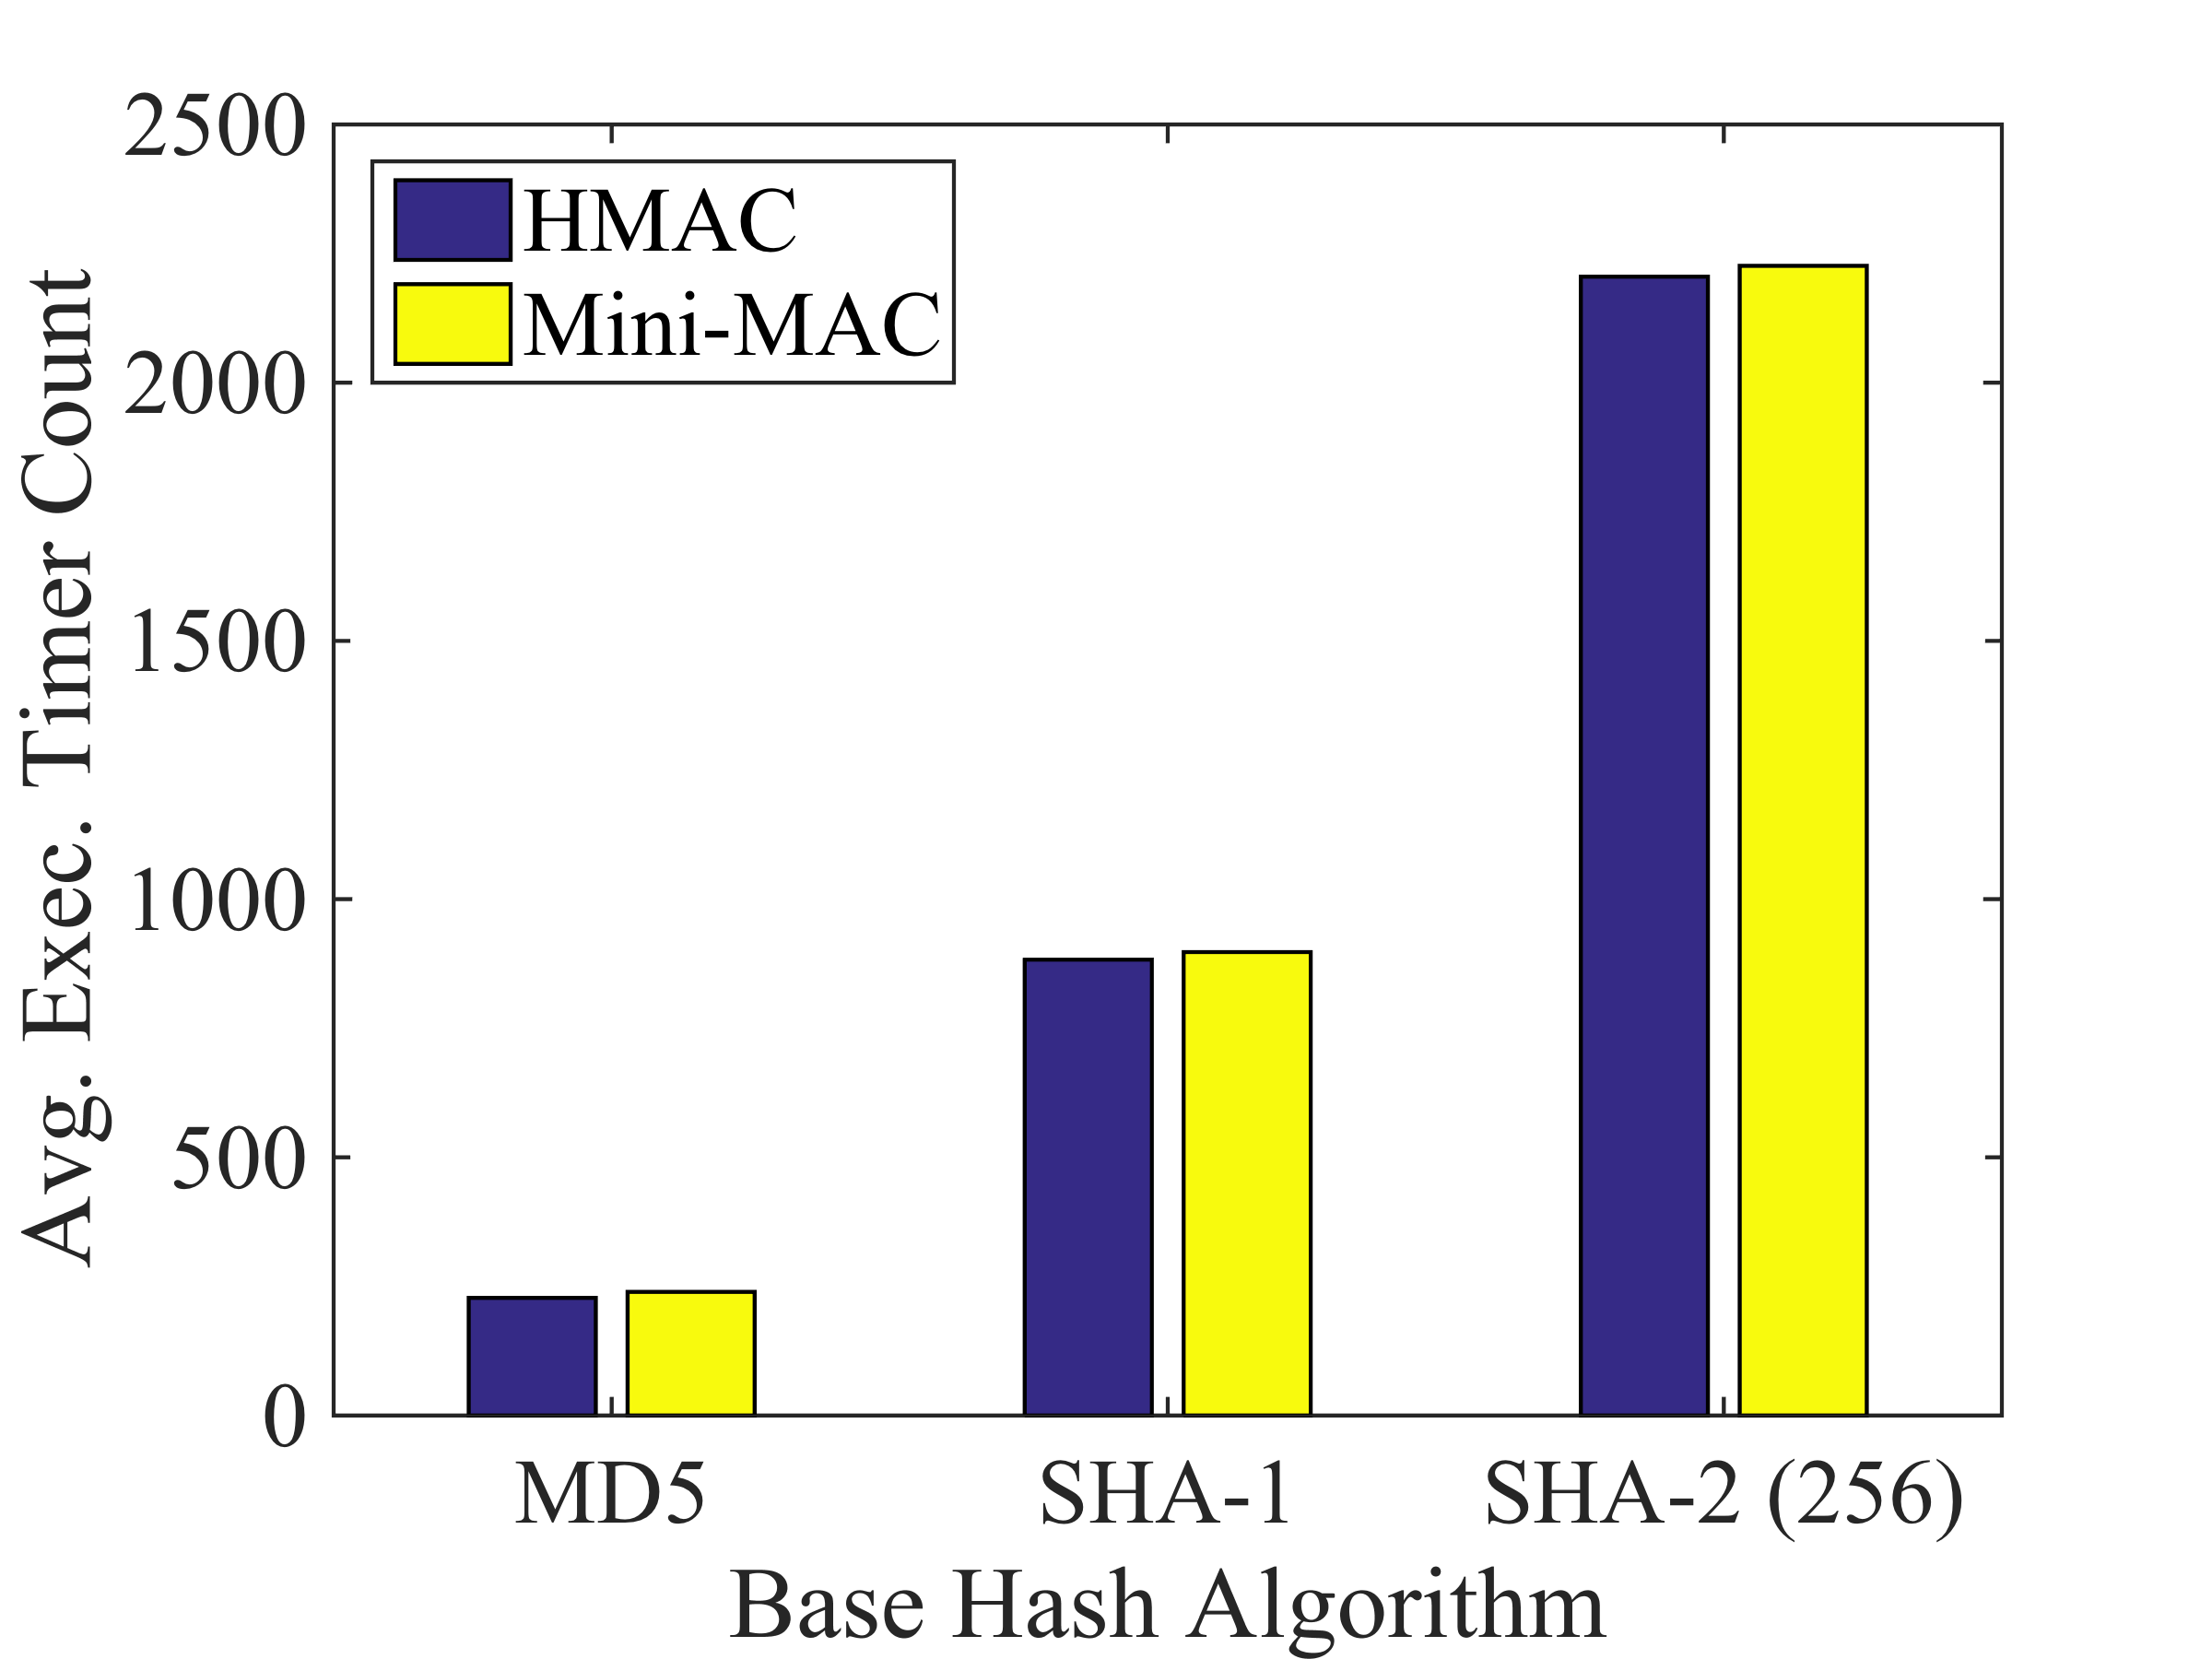
\includegraphics[width=\columnwidth]{figures/exec_cycles.png}
		\caption{Mean execution time for our Mini-MAC implementations, in cycles on a 32~kHz clock,
		from 1000 messages.}
		\label{fig-execution}
	\end{figure}
	
	\begin{figure}
		\centering
		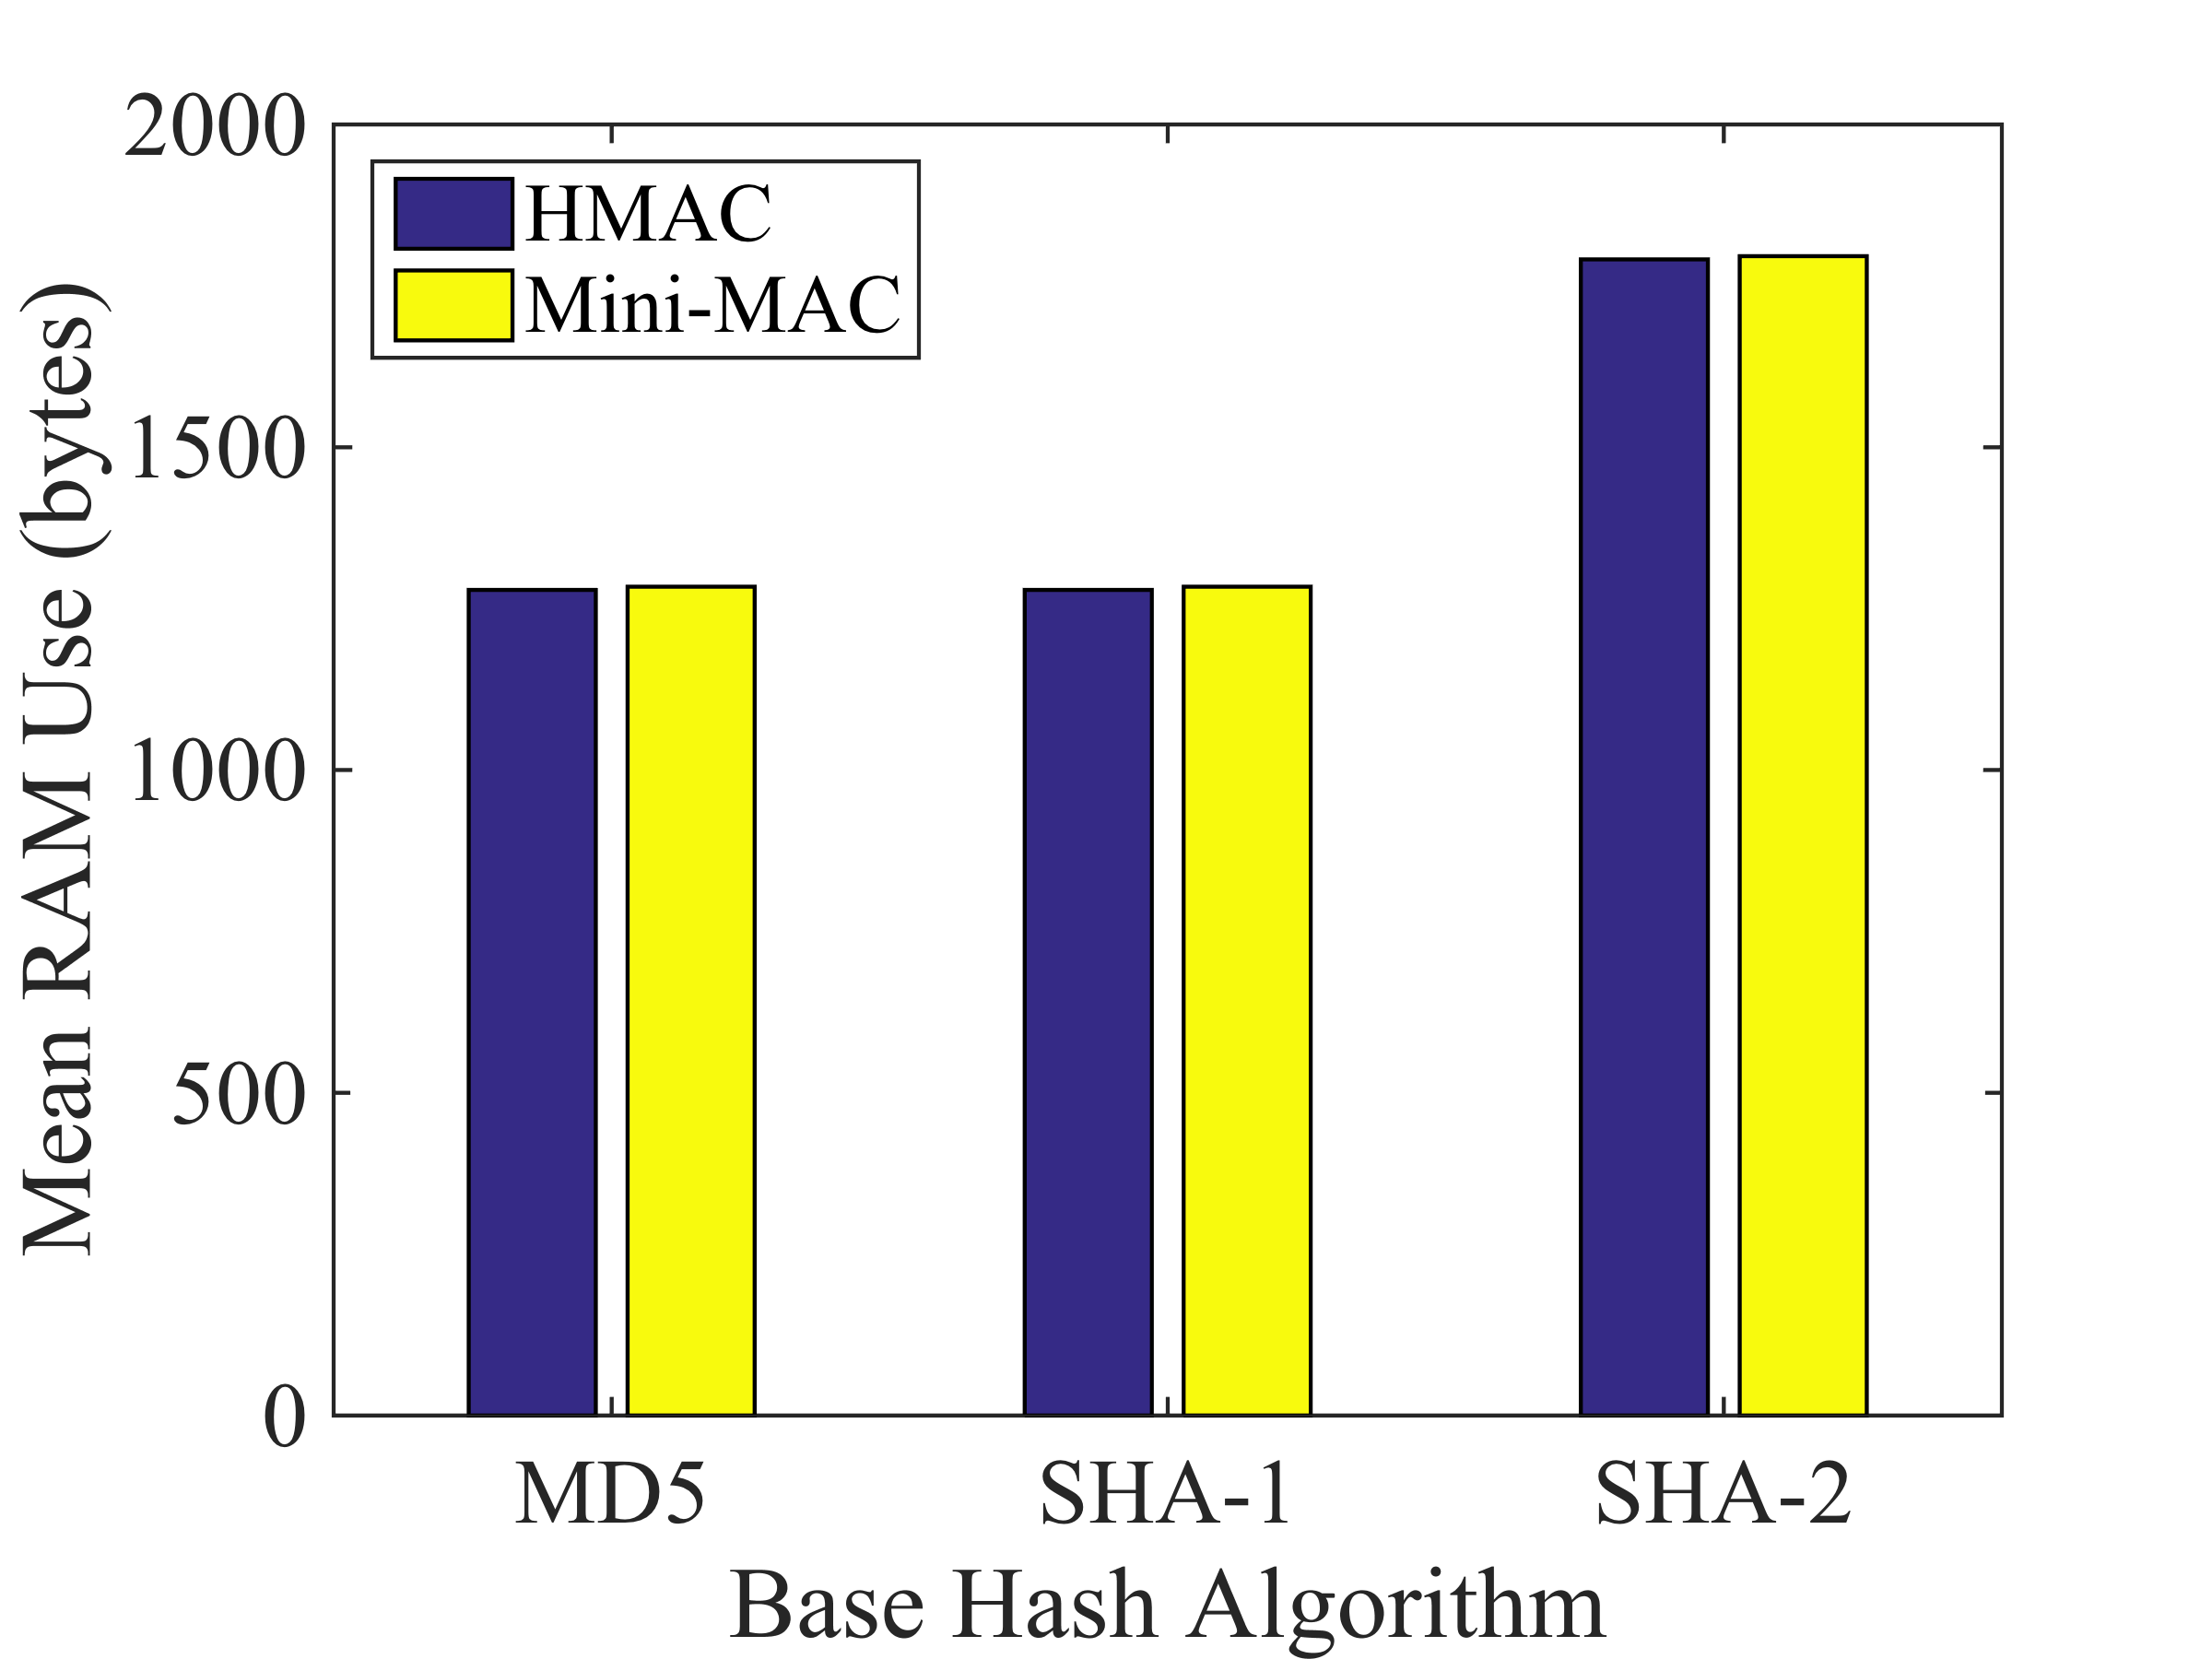
\includegraphics[width=\columnwidth]{figures/ram_usage.png}
		\caption{RAM usage for our Mini-MAC implementations, from 1000 messages.}
		\label{fig-ram}
	\end{figure}
	
	\begin{figure}
		\centering
		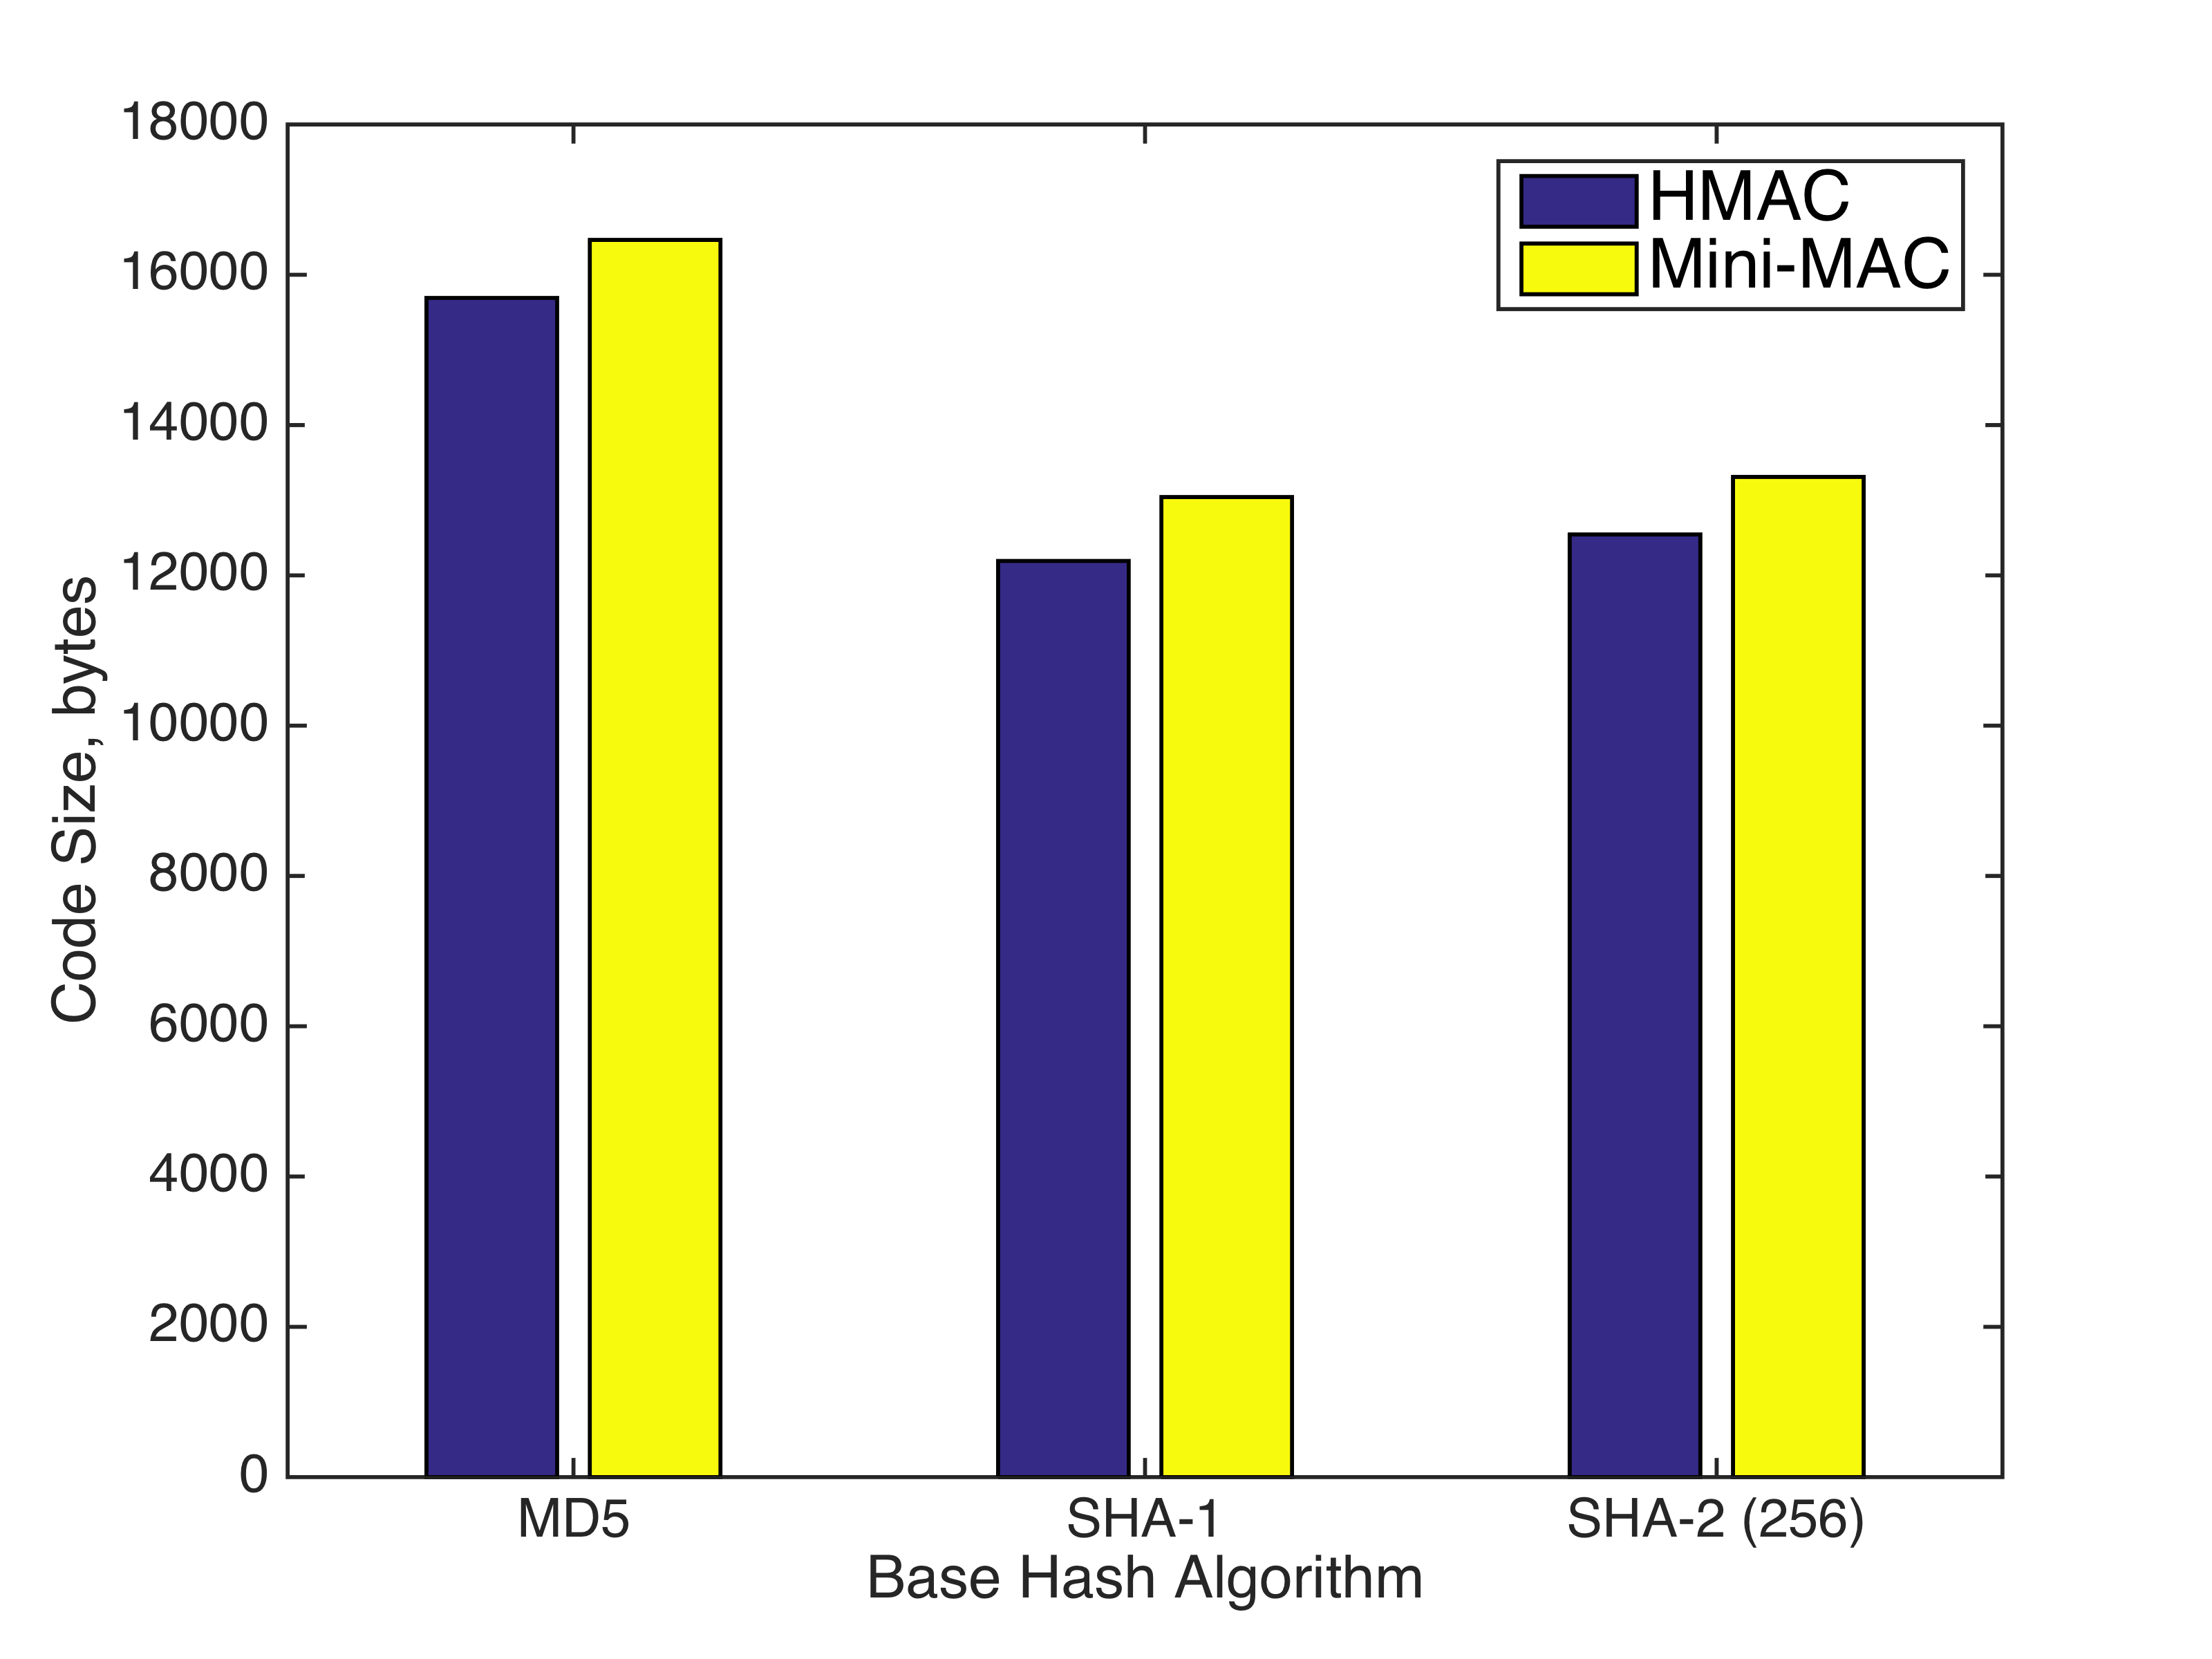
\includegraphics[width=\columnwidth]{figures/code_size.png}
		\caption{Code size of our Mini-MAC implementations.}
		\label{fig-code}
	\end{figure}
	
	
	

\section{Results and Analysis}
\label{analysis}

We analyze Mini-MAC for performance and authentication strength. 
Mini-MAC must be able to authenticate messages 
without compromising the performance of the real-time, safety-critical systems.

\subsection{Performance}
\label{performance}

Tables~\ref{tab-traffic}--\ref{tab-time} and Figures~\ref{fig-execution}--\ref{fig-code}
show the message traffic, execution time, code size, and RAM usage of our unoptimized implementations
of Mini-MAC and their underlying HMACs.  Time and space are dominated by the HMAC computation.

%Throughout, ``B''~denotes bytes, ``b''~denotes bits, and ``ms''~denotes milliseconds.

Table~\ref{tab-traffic} shows that Mini-MAC adds no additional bus traffic.
By contrast, HMAC-MD5 adds 128~bits (two CAN frames) per authentication,
due to the 128-bit tag.  Similarly, the pairwise-keyed Lin-MAC generates
two additional CAN frames per recipient ECU in each group communication.

Table~\ref{tab-time} shows the mean observed execution time
and standard deviation for each of our implementations of Mini-MAC.
Using MD5 is much faster than using SHA-1 or SHA-2.  As shown in Table~\ref{tab-overhead},
the overhead in time to compute Mini-MAC beyond HMAC is very little (approximately 0.38--0.68~ms).
Similarly, Figure~\ref{fig-execution} shows the mean observed execution times for Mini-MAC measured
in number of cycles on a 32~kHz clock.

Importantly, Table~\ref{tab-time} shows that only our 
MD5 implementation of Mini-MAC runs fast enough to satisfy our
requirement of authenticating at least 40 messages per second (approximately
25~ms between messages).   
While highly optimized code will likely run faster, on the
basis of our timing measurements, we recommend implementing Mini-MAC using MD5.

Figure~\ref{fig-ram} shows the RAM usage for our implementations of Mini-MAC.
As shown in Table~\ref{tab-overhead}, the overhead in RAM usage to compute Mini-MAC
beyond HMAC is very low (5~bytes).

Figure~\ref{fig-code} shows the code size of our Mini-MAC implementations.
As shown in Table~\ref{tab-overhead}, the additional code size for Mini-MAC beyond
HMAC is very small (approximately 800~bytes).
	
\subsection{Authentication Strength}
\label{security}

Mini-MAC detects spoofed messages by using a keyed HMAC.  It detects replay attacks
by incorporating a counter and recent message history into the HMAC input.  Using message
history also complicates a transient attacker who may be unable to observe a sufficient
number of recent messages.  

	\fontfamily{ptm}\selectfont
	\begin{figure}
		\centering
		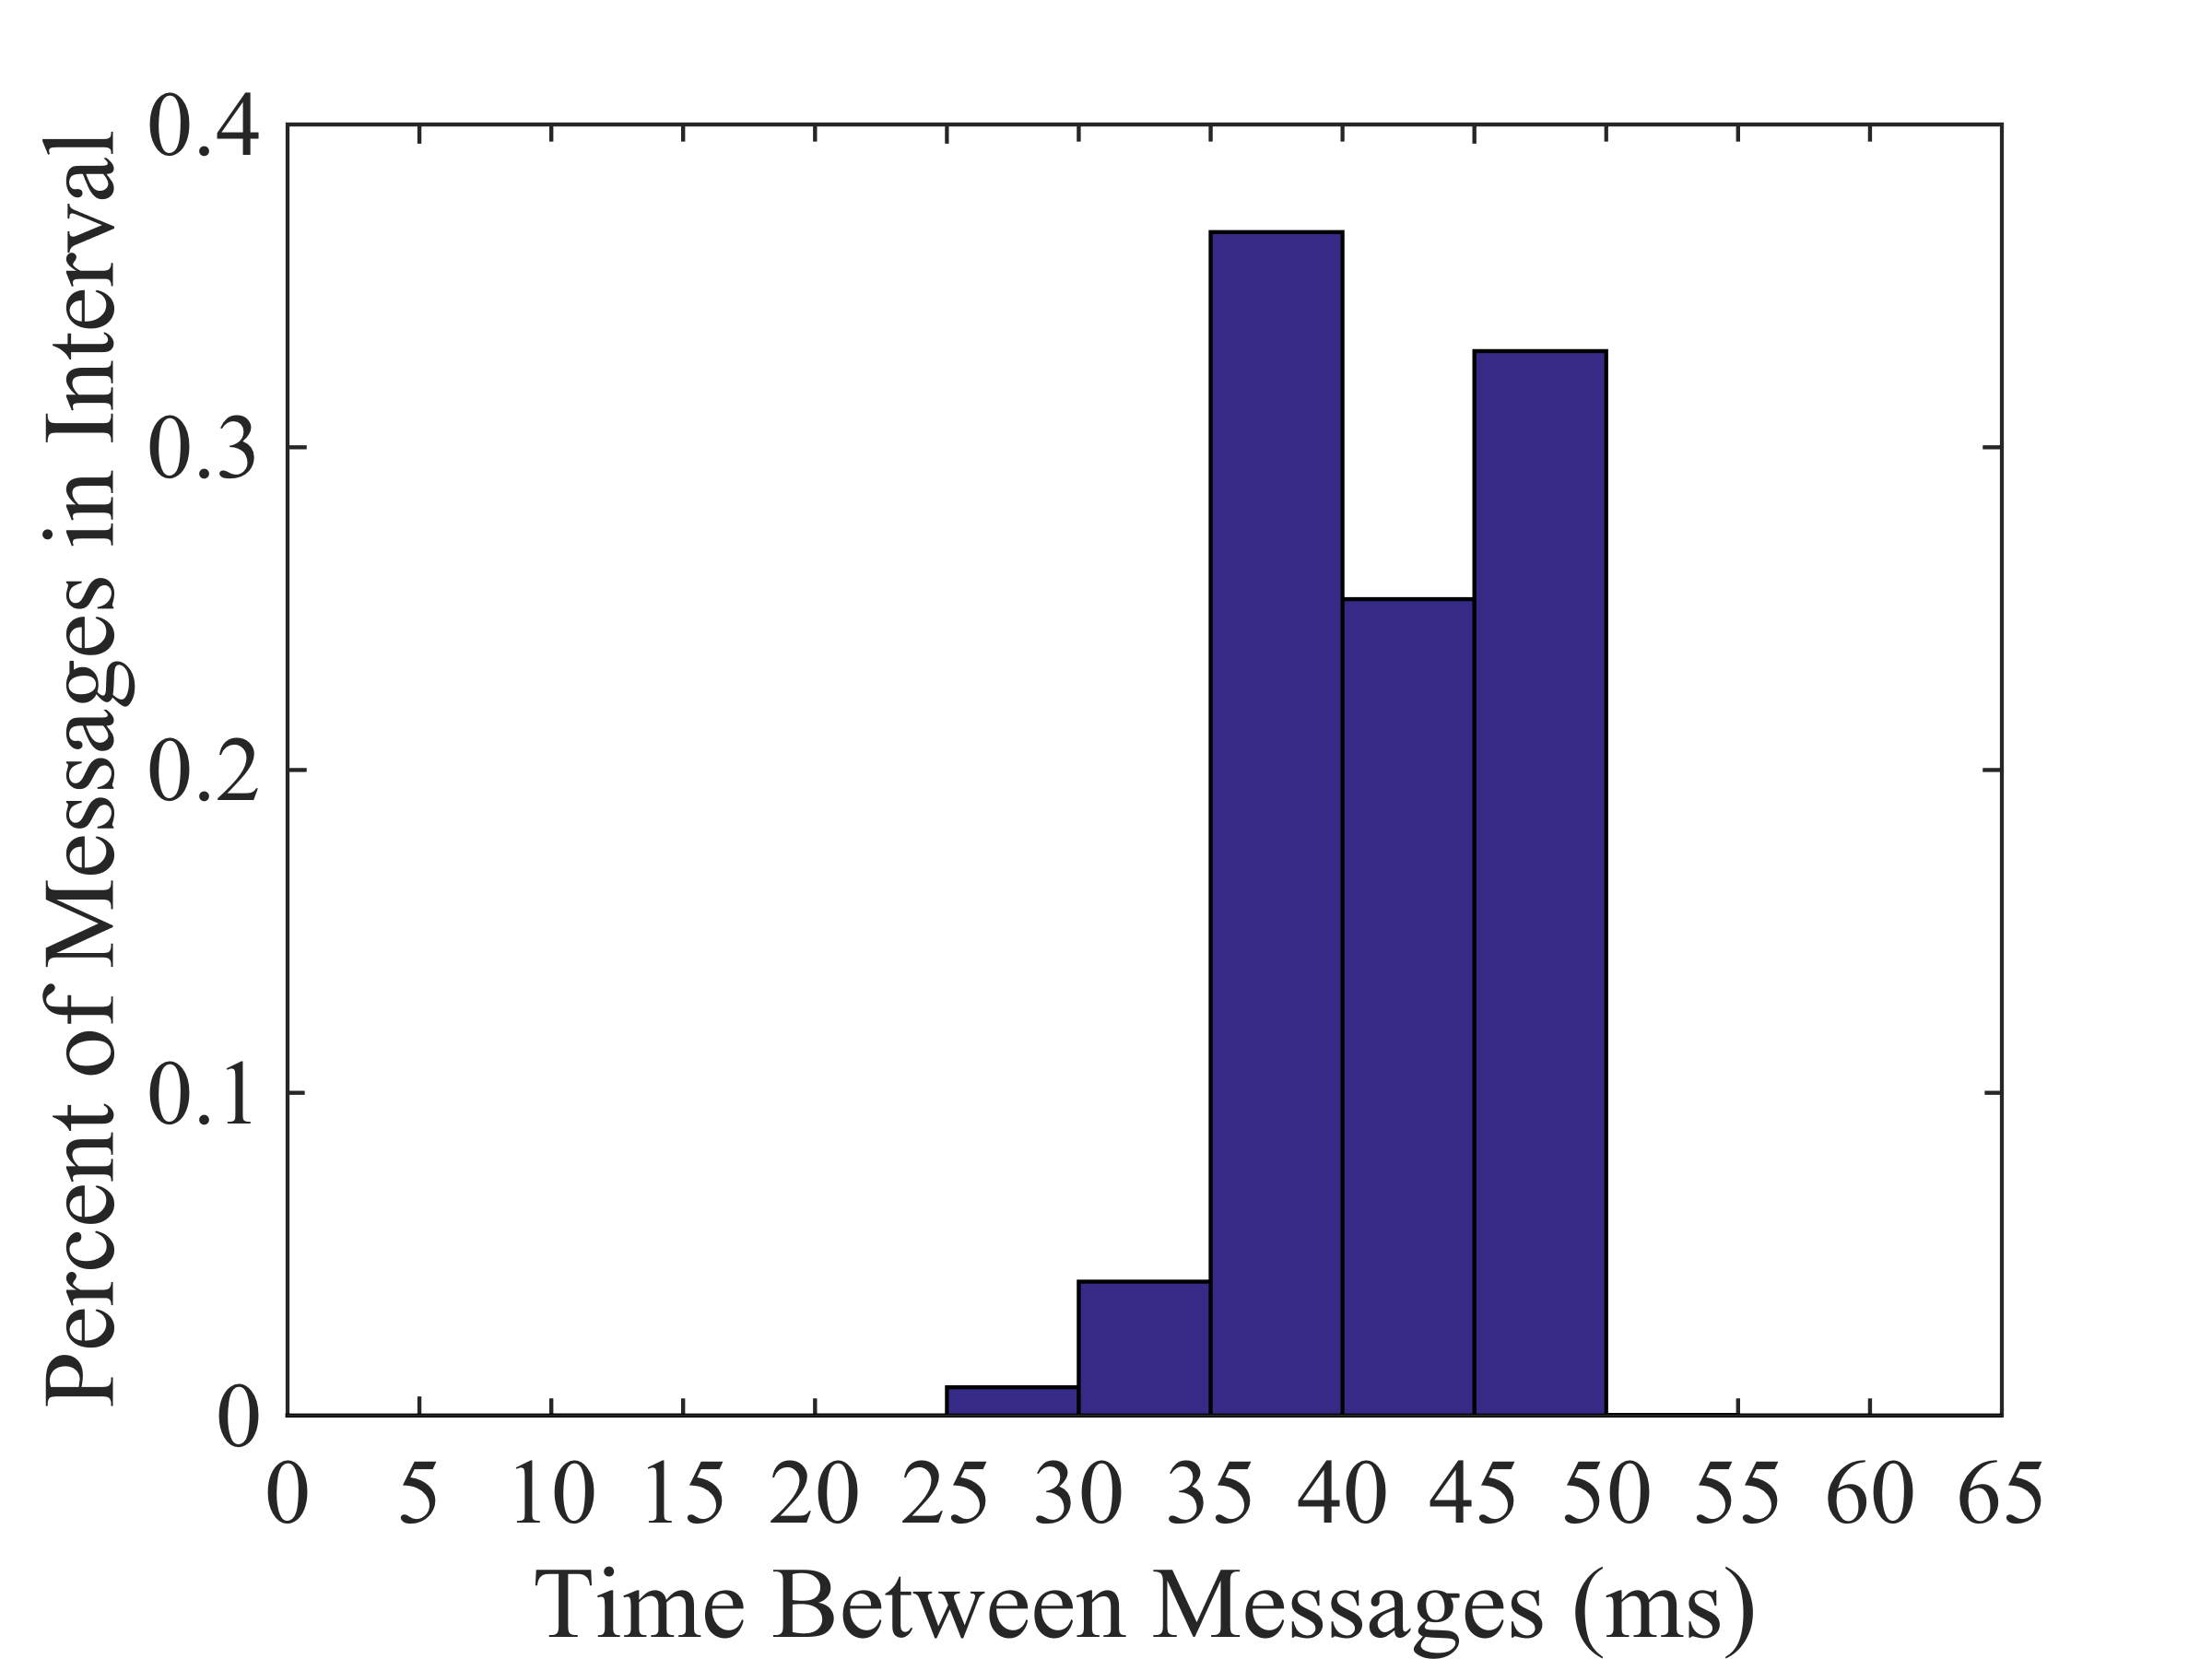
\includegraphics[width=\columnwidth]{figures/relative_histogram.png}
		\caption{{\fontfamily{ptm}\selectfont Histogram 
		of message interarrival times observed by the authors from 
		15,768 messages on a 2010 Toyota Prius. }}
		\label{fig-msgdelay}
	\end{figure}

\begin{table*}	
	\centering
	
	\caption{Probability and expected time for a spoofed message to be accepted by an ECU for various tag lengths
	for two attack scenarios.  In random guessing, the adversary guesses a tag.
	In the hypothetical collision search, the adversary seeks a Mini-MAC collision.
	Probability denotes the probability of success for one trial.
	Expected time denotes the expected time for the cumulative success probability to be~0.5.
	All calculations assume the adversary injects 40 forged messages per second.}
	
	\label{tab-taglength}
	\vspace{8pt}
	\begin{tabular}{c|rrl|rl}%
	{\bf Tag Length (bits)} & {\bf Random Guessing} &&& {\bf Collision Search} & \\
	& {\bf Probability} & {\bf Time} & & {\bf Time} & \\\hline
	8  & 0.0039 & 3.20 & sec & 0.40 & sec \\
	16 & 1.53\text{\sc{e}-}05 & 13.65 & min & 6.40 & sec \\
	24 & 5.96\text{\sc{e}-}08 & 58.25 & hour & 1.70 & min \\
	32 & 2.33\text{\sc{e}-}10 & 621.38 & day & 27.30 & min \\
	40 & 9.09\text{\sc{e}-}13 & 435.82 & year & 7.28 & hour \\
	48 & 3.55\text{\sc{e}-}15 & 111,568.9 & year & 4.85 & day \\
	\end{tabular}
	\end{table*}

The 128-bit keys are sufficiently long to withstand 
exhaustive key-search attacks.  The 64-bit counter is sufficient to prevent counter
rollover within the lifetime of the car.

With the enhanced message history feature, the adversary must learn a sample of
messages taken from a specified period of recent message history.  This period can be set
(e.g., 30~mins) to exceed the amount of time available for any transcient attacker.

A security-enhancing feature of the CAN bus is, ironically, its slow speed of at most
approximately 40 messages per second.  Figure~\ref{fig-msgdelay} shows a histogram of
message arrival times that we collected from a 2010 Toyota Prius.
The slow speed of the CAN bus limits the rate at which an attacker can
inject messages into the bus.

Another defensive feature is that there is no simple fast way for an adversary to
test if a candidate tag is valid.   The only way we are aware of is to inject a message into the bus
and observe if the receiving ECU accepted the message.

Limitations imposed by Mini-MAC include its use of group keys and truncated HMAC tags.  
Using group keys means that a single compromised ECU learns all of the keys
to which groups it belongs.  We consider this limitation an acceptable design tradeoff
given that Mini-MAC does not increase bus utilization and the compromise of any critical
ECU is a devastating security failure.

One potential attack is for the adversary to inject messages into the bus with the hopes
of trying a tag that verifies correctly.  We shall call this attack the ``trial injection attack.''
A downside of this attack is that it would be easy to detect such an attack involving
many messages.

Table~\ref{tab-taglength} lists for various tag lengths~$L$
two reference times that are useful in assessing the effectiveness of this and other hypothetical attacks.
The ``random guessing'' columns refer to the strategy of randomly guessing tags.
Probability denotes the probability that one guess will be accepted as valid; this probability
is $1/2^{L}$, where $L$ is the tag length.
Expected time denotes the expected time for the cumulative success probability to be~0.5,
assuming the adversary is limited to trying 40 tags per second.
This value is the expected time for a straight-forward 
implementation of a trial injection attack to succeed.  

The ``collision search'' column refers to an optimistic hypothetical attack whose success is based on
finding a Mini-MAC collision,\footnote{A collision is any pair of 
different inputs that produces the same output.}
exploiting the Birthday Paradox.  
We do not see how an adversary could mount such an attack;
we include this column simply as a conservative reference.

For example, with a four-byte tag, the expected time for a straight-forward 
message injection attack to succeed is over 621~days.  

Another potential attack is to observe bus traffic with the hopes of finding statistical
regularities that would significantly improve the chances of success of the aforementioned attack.
We conjecture that this attempt is unlikely to yield significant advantage, given the
strong properties of HMAC and some
desirable (albeit imperfect) characteristics of the component hash functions.

Given that the CAN bus does not authenticate messages, we conclude that Mini-MAC
meaningfully raises the bar of vehicular security.


	

	
\section{Discussion}
\label{discuss}

In this section we discuss how to resynchronize ECUs, 
how to lengthen the mini-MAC tag as an optional improvement, 
and we list some open problems.

%a radical design alternative, 

\subsection{Resynchronization}
\label{resynch}

Our mini-MAC proposal requires the ECUs to have synchronized counters and message-history states.
Therefore, a mechanism is needed to resynchronize the ECUs in case they ever lose synchronization,
as might happen, for example, by a fault in the ECU or a disruption in message transmission.

Two common solutions are to reset the state to a specified initial state, or for one ECU to select
a new state and communicate that state to the other ECUs (encrypted by a shared secondary communication
encryption key).  [do you have a ref?]

Instead, for enhanced security we propose that each ECU periodically save its state in persistent memory.  
In the initial attempt to resynchronize, each ECU loads its most recent state.  If that fails, then the aforementioned
mechanisms could be applied.  Section~\ref{arch} explains how message history helps guard against
replay attacks upon resynchronization.

A limitation of the CAN bus is that it provides no mechanism for detecting when ECUs are out
of synchronization.  In some cases, by monitoring observable conditions on the bus, 
an ECU might detect that another ECU is not responding to a message, which might be
the result of a synchronization failure.  A tradeoff in our design is that, by using
counters and message history to athenticate messages, 
mini-MAC increases the opportunities for possible synchronization failures.

%% this section is rather weak--nothing new.  No anlysis of proposal.
%% It is good to mention need for resynch.  We should not claim any contribution here.

\subsection{Lengthening the Mini-MAC Tag}
\label{addingbits}

Optionally, it is possible to lengthen the Mini-MAC tag by 
using the two bytes of space allocated for the CRC field in the CAM frame (see Figure~\ref{fig-frame}),
as suggested by Woo et al.~\cite{Woo-14} in a related proposal.
Because a MAC detects transmission errors (in fact, better than a simpler CRC), there is no need for
a CRC in addition to a MAC.  [explain fig. note that it is based on birthday calcs, which is not
exactly right]

Increasing the tag length greatly increases the time required for an adversary to forge a valid tag by
finding a collision in the Mini-MAC by exhaustive search.  
Table~\ref{tab-taglength} gives the expected time for an adversary to send a forged message 
that will be accepted by another ECU, for various tag lengths.  Here, the main limiting assumption is 
the frequency with which messages can be sent on the CAN bus 
(approximately 25 messages per second. [in table, change b to bits]
For example, increasing the tag from 32 to 48 bits increases this time from
approximately 27.3~minutes to over four days.

%% as we will point out in the security section, exchaustive search attacks to finds collisions are
%% not so useful because there is no way for the adversary to check candidate values.
%% perhaps the best attack is just to inject many messages, hoping one will work, an attack
%% which could be easily detected

To implement this strategy one could modify the lower-level code in the CAN network stack, 
either to perform the MAC calculation there 
or to open the CRC field to the application level to calculate the MAC.

%% compare with Woo (see previous work).
%% we are not first to suggest.  How do we differ?
%% it is a bit lame to emphasize that we are optional and woo is not.

	\begin{table}	
	\centering
	\caption{Expected time for some spoofed message to be accepted by an ECU for various tag lengths, 
	assuming the adversary injects 40 forged messages per second.[add col for linear search]}
	\label{tab-taglength}
	\vspace{8pt}
	\begin{tabular}{c|r}%
	\bfseries Tag Length (b) & \bfseries Time to Find Collision\\\hline \csvreader[late after line=\\]%
		{tables/maclen_bfttb.csv}{mac_len=\mac_len,ttb=\ttb}% 
		{\mac_len & \ttb}%
	\end{tabular}
	\end{table}
	
	%% I don't know this mechanism. need to add space between number and unit in each line
	%% headers should be done in latex directly

%\subsection{Design Alternative}
%\label{alternatives}

%% would be nice to discuss our enigneering decisions and alternatives, but we don't have anything interesting to say

\subsection{Open Problems}
\label{open}

Our engineering decisions are driven by a desire to improve vehicular security by adding authentication
to the CAN bus, without increasing bus traffic or delaying messages, and without making any
disruptive changes.  The egregious state of vehicular security, however, demands a radical disruptive
redesign of vehicular computer networks carried out including security as a foundational design
requirement. [should we cite any discussion like this from someone else?  are we the first to say so?]

Design ideas for a replacement network to the CAN bus include the following:  
(1)~Use a well-established high-speed network (such as 802.3 Ethernet) on which
standard security mechanisms (such as IPsec) can be deployed.
(2)~Segegrate nodes on the bus into task-defined groups.
(3)~Protect access to the bus by physically separating critcal and non-critical systems.
In particular, it should not be possible for maleware or faults in entertainment or 
Bluetooth systems to affect braking, steering, or acceleration.  

A separate related problem is to detect vehicular network intrusions. [ref?]  A challenge of such work is that
there is no good reponse of what to do if an intrusion is detected other than to shut down the vehicle safely.

The Car-to-X network~\cite{C2X} is an emerging interconnected collection of vehicles, buildings, signs, and road infrastructure 
to reduce congestion and enable more efficient traffic control. Cars of the future will have to be able to communicate
securely with objects on such networks, requiring authentication and key management beyond Mini-MAC.

%% I don't think the draft question about padding or security of truncated MACs is in a state worthy of mention here.



\section{Conclusion}
\label{conclude}

We propose Mini-MAC, the first variable-length message authentication
protocol for the CAN bus that neither increases the number of messages sent
nor delays any message,
allowing it to be used in vehicular systems with time-sensitive messages.  
The truncated keyed HMAC protects against
message injection by adversaries who do not know the ECU keys.  
The counter and message history protect against replay attacks.  
Message history also protects against all transient attackers, even if they know the authentication keys.

Limited message size, the need not to delay messages, the limited computational power of the ECUs,
and the relative ease of gaining access to the bus severely restrict how well the CAN bus can be protected.  
Mini-MAC meaningfully raises the bar on vehicular security,
approaching (we conjecture) the limits of what is possible for authentication strength in this highly
constrained environment.

Objects and systems in the emerging Internet of Things and Car-to-X network
will face similar authentication challenges to those faced by 
vehicular ECUs.  We hope, for example, that the designers of toaster ovens will not
separately create ad-hoc security mechanisms for networked communications with
the refrigerator, home electrical system, home owner, and toaster manufacturer.
Instead, networked objects of the future need to be built with 
control units that can execute resilient general-purpose standard cryptographic 
functions and protocols suitable for the Internet of Things.  We hope that some
of the ideas from Mini-MAC will be helpful toward that objective.





\section{Acknowledgments}

% Redacted.

Schmandt and Sherman were supported in part by the 
National Science Foundation (NSF) under SFS grant 1241576. 
Sherman was also supported under a subcontract of NSF INSuRE grant 1344369, 
and by the Department of Defense under CAE-R grant H98230-15-10294.
Banerjee was supported in part by NSF under awards 
CPS-1544687, CNS-1305099, IIS-1406626, CNS-1308723, and CNS-1314024, 
and by Microsoft under a SEIF Award.
Any opinions, findings, conclusions, or recommendations expressed 
are those of the authors and do not necessarily reflect the views
of the sponsors.

\clearpage
\bibliography{mybib}
\bibliographystyle{alpha}

\bigskip \noindent
Preliminary draft to be submitted to {\it Cryptologia}. {\today}.

\end{document}


